%template by Marcel Neunhoeffer & Sebastian Sternberg - Uni of Mannheim

\documentclass[a4paper, 12pt]{article}  %khai bao document class

% set up margin
\usepackage[top = 2.5cm, bottom = 2.5cm, left = 2.5cm, right = 2.5cm]{geometry} 
% \usepackage[utf8]{inputenc}  % language encoder
\usepackage[utf8]{vietnam}  % vietnamese language setting
\usepackage{multirow} % Multirow is for tables with multiple rows within one cell.
\usepackage{booktabs} % For even nicer tables.
\usepackage{graphicx}
\usepackage{ulem} % for underlined format
% packages for advanced math eqn and symbols
\usepackage{amsmath}
\usepackage{amssymb}
\usepackage{amsthm}
\usepackage{enumitem} % for itemize
\usepackage{hyperref}

% set indent of new paragraph to 0
\usepackage{setspace}
\setlength{\parindent}{0 in}
\onehalfspacing

% Package to place figures where you want them.
\usepackage{float}

% The fancyhdr package let's us create nice headers.
\usepackage{fancyhdr}

%%Make header and footer
\pagestyle{fancy} % With this command we can customize the header style.
\fancyhf{} % This makes sure we do not have other information in our header or footer.

% Header
\lhead{\footnotesize Machine Learning 1: Homework 4}% \lhead puts text in the top left corner. \footnotesize sets our font to a smaller size.
\rhead{\footnotesize Nguyen Anh Tu @DSEB 62}

% Similar commands work for the footer (\lfoot, \cfoot and \rfoot).
% We want to put our page number in the center.
\cfoot{\footnotesize \thepage} 

%%%%%%%%%%%%%%%%%%%%%%%%%% 
\begin{document}

% Title section of the document
\thispagestyle{empty} % This command disables the header on the first page. 

\begin{tabular}{p{12.5cm}} % This is a simple tabular environment to align your text nicely 
{\large \bf National Economics University, Vietnam} \\
Faculty of Mathematics Economics \\ Data Science in Economics and Business  \\ Machine Learning 1\\
\hline % \hline produces horizontal lines.
\\
\end{tabular} % Our tabular environment ends here.

\vspace*{0.3cm} % Now we want to add some vertical space in between the line and our title.

\begin{center} % Everything within the center environment is centered.
	{\Large \bf Homework Week 4} % <---- Don't forget to put in the right number
	\vspace{2mm}
	
	{\bf Student: Nguyễn Anh Tú - ID: 11207333} % <---- Fill in your names here!
\end{center}  

%%%%%%%%%%%%%%%% Problem 1:
\section{Problem 1}

Fit model Parabola Linear Regression cho tập dữ liệu \href{https://github.com/nttuan8/DL_Tutorial/blob/master/L1/data_square.csv}{data\_square.csv}:

%%%% Solution
\textbf{Solution.} 

Mô hình được sử dụng là Parabola Linear Regression vì vậy giả thiết (hypothsis) được đưa ra như sau:
\[y = w_0 + w_1 x + w_2 x^2\]

Dataset cho sẵn chỉ chứa hai cột giá trị x và y nên code đã được xây dựng để thêm cột chứa giá trị của $x^2$. Ta có thể coi $x^2$ lúc này như một biến độc lập mới trong mô hình của mô hình Linear Regression. Huấn luyện mô hình này sử dụng kết quả của Normal Equation, ta được kết quả các hệ số như sau:
\begin{align*}
    w_0 &= 2.00000579e+03 \\
    w_1 &= 1.00000199e+00 \\
    W_2 &= -1.00000222e+02
\end{align*}

Đường dự đoán và dữ liệu được vẽ trên đồ thị scatter như sau:
\begin{center}
    \includegraphics[width=0.7\linewidth]{Problem 1 HW4.png}
\end{center}
    
    
%%%%%%%%%%%%%%%%%%%%% Problem 2:
\section{Problem 2}

Tự sinh dữ liệu như hình sau:
\begin{center}
    \includegraphics{Problem 2 HW4.png}
\end{center}

\begin{enumerate}[label=\alph*.]
    \item Fit dữ liệu trên với các mô hình Linear Regression của đa thức bậc 0, 1, 3, 6, 9, vẽ mô hình và nhận xét mô hình.
    \item Thêm 15 và 100 điểm dữ liệu vào dữ liệu ban đầu và chạy thử mô hình đa thức bậc 9. Nhận xét mức độ overfitting của mô hình.
    \item Fit đa thức bậc 9 cho 10 điểm dữ liệu ban đầu nhưng dùng Ridge Regression và Lasso Regression để tránh overfitting.
\end{enumerate}

\textbf{Solution.} 
\begin{enumerate}[label=\alph*.]
    \item Các mô hình được xây dựng tương tự như mô hình bậc 2 của Problem 1, code đã được xây dựng để sinh thêm dữ liệu cho các lũy thừa của $x$ cho những mô hình có bậc cao. Với mô hình bậc 0, giả thiết được đưa ra là \(y = \overline Y \), hay chính là giá trị trung bình của dữ liệu biến $y$.
    
    Đường dự đoán và dữ liệu được vẽ trên đồ thị scatte của từng mô hình như sau:
    
    \begin{figure}[H]
        \centering
        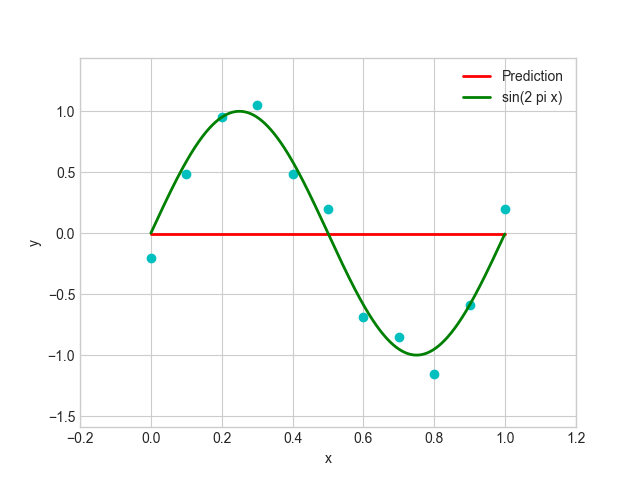
\includegraphics[width=0.6\linewidth]{Problem 2 part a model order 0.png}
        \caption{Mô hình bậc 0: $y = \overline Y$}
        \label{fig:Data1}
        
        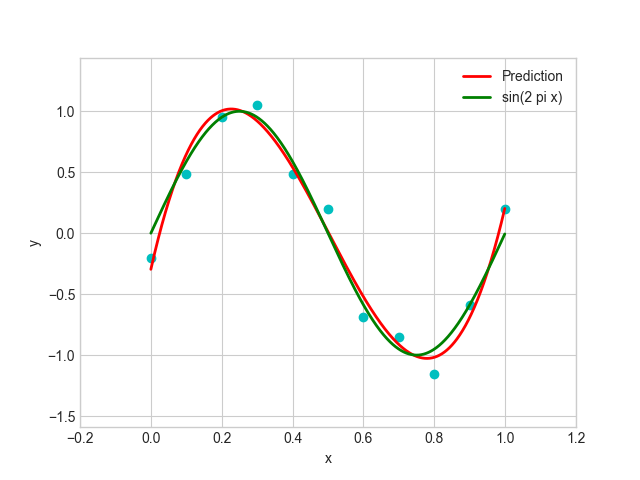
\includegraphics[width=0.6\linewidth]{Problem 2 part a model order 3.png}
        \caption{Mô hình bậc 3 linear regression, n = 10}
        \label{fig:Data2}
    \end{figure}
    \begin{figure}[H]
        \centering
        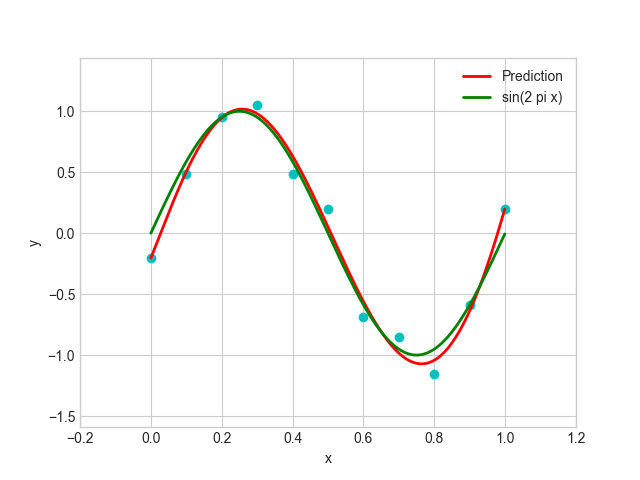
\includegraphics[width=0.6\linewidth]{Problem 2 part a model order 6.png}
        \caption{Mô hình bậc 6 linear regression, n = 10}
        \label{fig:Data3}
    \end{figure}
    
    \begin{figure}[H]
        \centering
        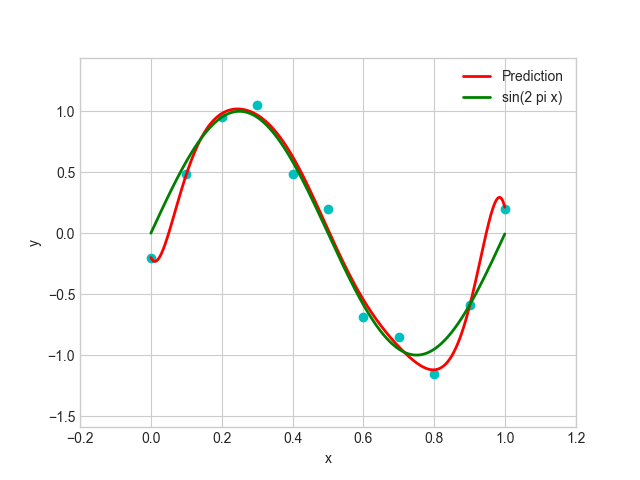
\includegraphics[width=0.6\linewidth]{Problem 2 part a model order 9.png}
        \caption{Mô hình bậc 9 linear regression, n = 10}
        \label{fig:Data4}
    \end{figure}
    
    \textbf{Nhận xét.} Do dữ liệu về $x$ và $y$ được xây dựng theo hàm \(y = \sin (2 \pi x + \text{noise})\), ngoài đường dự đoán màu đỏ thể hiện các giá trị dự đoán của mô hình, các đồ thị còn chứa đường hồi quy chuẩn \(y = \sin (2 \pi x)\) màu xanh để tiện so sánh kết quả dự đoán:
    \begin{itemize}
        \item Mô hình bậc 0 thể hiện rằng $y$ không bị phụ thuộc bởi $x$. Đồ thị cho thấy mô hình này không khớp với đường hồi quy chuẩn do quá đơn giản. Mô hình này gặp phải tình trạng underfitting.
        \item Mô hình bậc 3 và bậc 6 có đường dự đoán trùng khớp ở mức cao với đường hồi quy chuẩn. Tuy nhiên mô hình bậc 3 có sự cân bằng nhiều hơn một chút giữa các giá trị của $x$, mô hình bậc 6 khớp với dữ liệu hơn nhưng đó là dấu hiệu của overfitting nhẹ.
        \item Mô hình bậc 9 khớp gần như hoàn toàn vớ 10 điểm dữ liệu nhưng không có sự khớp nhiều với đường hồi quy chuẩn như hai mô hình trước. Mô hình này gặp phải tình trạng overfitting.
    \end{itemize}
    
    \item Sau khi bổ sung thêm điểm dữ liệu vào mô hình bậc 9, kết quả đường dự đoán được thể hiện như sau:
    \begin{figure}[H]
        \centering
        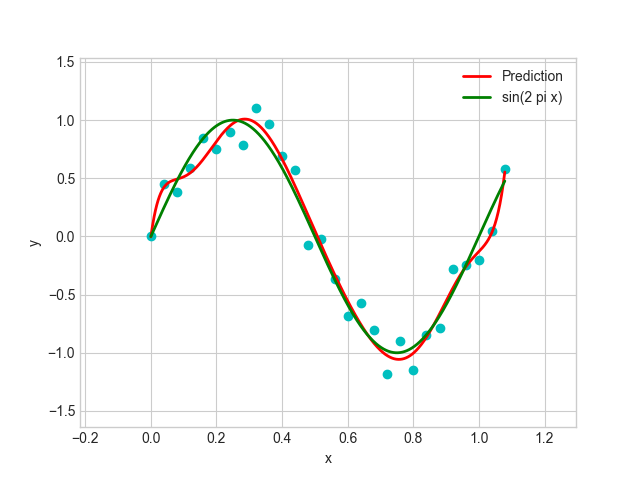
\includegraphics[width=0.6\linewidth]{Problem 2 part b small.png}
        \caption{Mô hình bậc 9 linear regression, n = 25}
        \label{fig:Data5}
    \end{figure}
    
    \begin{figure}[H]
        \centering
        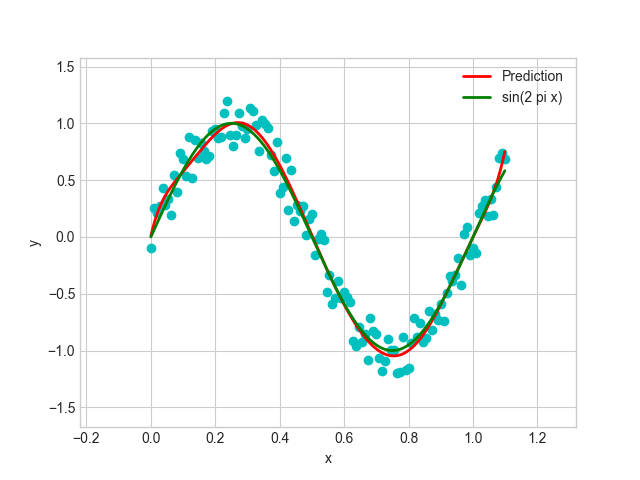
\includegraphics[width=0.6\linewidth]{Problem 2 part b large.png}
        \caption{Mô hình bậc 9 linear regression, n = 110}
        \label{fig:Data6}
    \end{figure}
    
    \textbf{Nhận xét.} Kết quả dự đoán của mô hình bậc 9 đã được cải thiện rất nhiều khi bổ sung thêm các điểm dữ liệu vào mô hình. Đặc biệt khi bổ sung thêm 100 điểm dữ liệu, đường dự đoán tuy không khớp nhiều với dữ liệu $x$ nhưng có sự khớp gần như hoàn toàn với đường hồi quy chuẩn.
    
    \item Đầu tiên cần xây dựng lý thuyết cách huấn luyện cho mô hình sử dụng Ridge Regression và Lasso Regression.
    
    Với Ridge Regression, hàm mất mát được định nghĩa lại như sau:
    \[\mathcal{L}(w) = \frac{1}{N} ||xw - y||^2_2 + \alpha||w||_2^2 
    = \frac{1}{N} (xw - y)^T (xw - y) + \alpha w^T w\]
    Để tìm được nghiệm tối ưu cho hàm mất mát trên, lấy đạo hàm riêng theo $w$ của $\mathcal{L}(w)$ ta được:
    \begin{align*}
        \frac{\partial \mathcal{L}(w)}{\partial w} &= \frac{1}{N} \frac{\partial (xw - y)^T (xw - y)}{\partial w} + \alpha \frac{\partial w^T w}{\partial w}\\
        &= \frac{2}{N} x^T (xw - y) + 2\alpha w \\
        &= \frac{2}{N} [(x^T x + N \alpha \mathbf{I})w - x^T y]
    \end{align*}
    
    Nghiệm tối ưu được tìm ra khi giải phương trình:
    \begin{align*}
        \frac{\partial \mathcal{L}(w)}{\partial w} = 0 &\Longleftrightarrow \frac{2}{N} [(x^T x + N \alpha \mathbf{I})w - x^T y] = 0\\
        &\Longleftrightarrow (x^T x + N \alpha \mathbf{I})w = x^T y\\
        &\Longleftrightarrow w = (x^T x + N \alpha \mathbf{I})^{-1} x^T y
    \end{align*}
    Áp dụng kết quả trên để tìm vector hệ số cho mô hình, ta được đồ thị dữ liệu và đường dự đoán như sau:
    \begin{figure}[H]
        \centering
        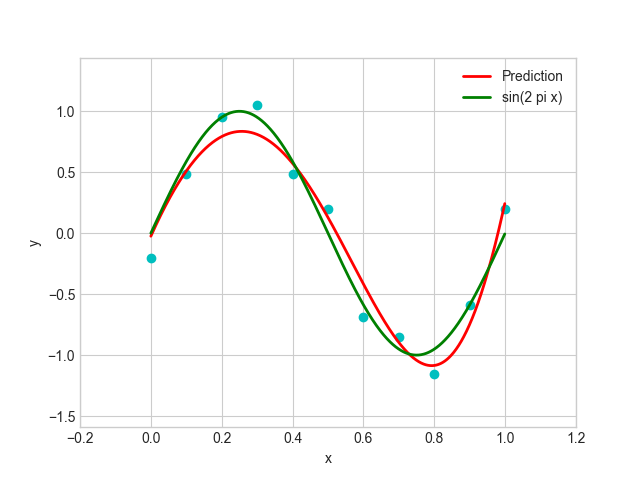
\includegraphics[width=0.6\linewidth]{Problem 2 Ridge Regression.png}
        \caption{Mô hình bậc 9 Ridge Regression, n = 10, $\alpha = 0.0001$}
        \label{fig:Data7}
    \end{figure}
    Hình trên cho thấy dù với bộ dữ liệu chỉ chứa 10 điểm, tình trạng overfitting của mô hình bậc 9 được cải thiện hoàn toàn.
    
    Với Lasso Regression, hàm mất mát được định nghĩa như sau:
    \[\mathcal{L}(w) = \frac{1}{N} ||xw - y||^2_2 + \lambda||w||_1 
    = \frac{1}{N} (xw - y)^T (xw - y) + \lambda \sum^N_i |w_i|\]
    
    Hàm mất mát kể trên không có đạo hàm liên tục, vì vậy ta sẽ sử dụng phương pháp Gradient Descent để tìm nghiệm tối ưu cho hàm mất mát trên. Vector gradient của $\mathcal{L}(w)$ như sau:
    \begin{align*}
        \nabla \mathcal{L}(w) &= \frac{2}{N} x^T (xw - y) + \lambda \nabla ||w||_1 \\
        &= \frac{2}{N} x^T (xw - y) + \lambda \frac{\partial ||w||_1}{\partial w_i} \sum^N_i |w_i| \\
        &= \frac{2}{N} x^T (xw - y) + \lambda \cdot sign(w)
    \end{align*}
    Cách học của thuật toán Gradient Descent như sau: \(w_{k+1} = w_k + \alpha \nabla \mathcal{L}(w)\). Vòng lặp trên sẽ kết thúc khi chuẩn vector (vector norm) của gradient vector nhỏ hơn một sai số $\epsilon$ nào đó.
    Đồ thị và đường dự đoán của mô hình bậc 9 sử dụng Lasso Regression như sau:
    \begin{figure}[H]
        \centering
        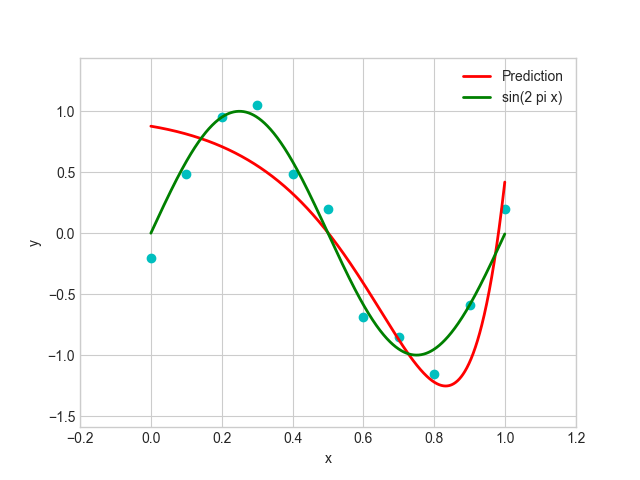
\includegraphics[width=0.6\linewidth]{Problem 2 Lasso Regression.png}
        \caption{Mô hình bậc 9 Lasso Regression, n = 10, $\lambda = 0.045, \epsilon = 0.1, w_0 = 0$, learning rate = 0.1}
        \label{fig:Data8}
    \end{figure}
    Đồ thị trên cho thấy vấn đề overfitting đã được giải quyết hoàn toàn, nhưng kết quả chưa tốt bằng Ridge Regression.
\end{enumerate}
\end{document}
